\chapter{PLL (Phase-Locked Loop)}

\section*{Resumen}

Un Lazo de Seguimiento de Fase, conocido universalmente por sus siglas en inglés PLL (\textit{Phase-Locked Loop}), existe desde hace muchas décadas. En el contexto de este informe, se utilizará para generar una o más frecuencias de salida. Por lo general, los componentes que generan directamente una frecuencia de salida ajustable no suelen ser tan estables ni presentar un nivel de ruido tan bajo como una entrada de frecuencia fija. Por ello, mediante el uso de realimentación (como la que emplea el PLL) resulta posible obtener una frecuencia ajustable con gran precisión y un excelente rendimiento en cuanto a ruido \cite{Dean Banerjee}.

\section{Principio de funcionamiento}

Como se puede observar en la Figura~\ref{fig:fig4.1} del diagrama de bloques, el funcionamiento del PLL comienza con una frecuencia de entrada estable ($f_{OSC}$). Un divisor $R$ reduce esta señal hasta alcanzar la frecuencia del detector de fase ($f_{PD}$).

Posteriormente, el detector de fase-frecuencia compara la fase resultante del divisor $R$ ($f_{PD}$) con la fase proveniente del divisor $N$ ($f_N$). Como resultado, genera pulsos de corrección de corriente cuyo ciclo de trabajo es proporcional al error de fase entre ambas entradas del detector. Estos pulsos tienen tres estados posibles: suministrar corriente ($K_{PD}$), absorber corriente ($K_{PD}$) o permanecer apagados (triestado).

La bomba de carga puede modelarse como una fuente de corriente analógica. Su función es generar una corriente cuya magnitud equivale a $K_{PD}$ multiplicada por el error de fase presentado al detector.

Finalmente, estos pulsos de corrección de corriente atraviesan un filtro paso bajo, conocido como filtro de bucle, el cual posee una función de transferencia de corriente a voltaje denotada como $Z(s)$.

\begin{figure}[H]
    \centering
    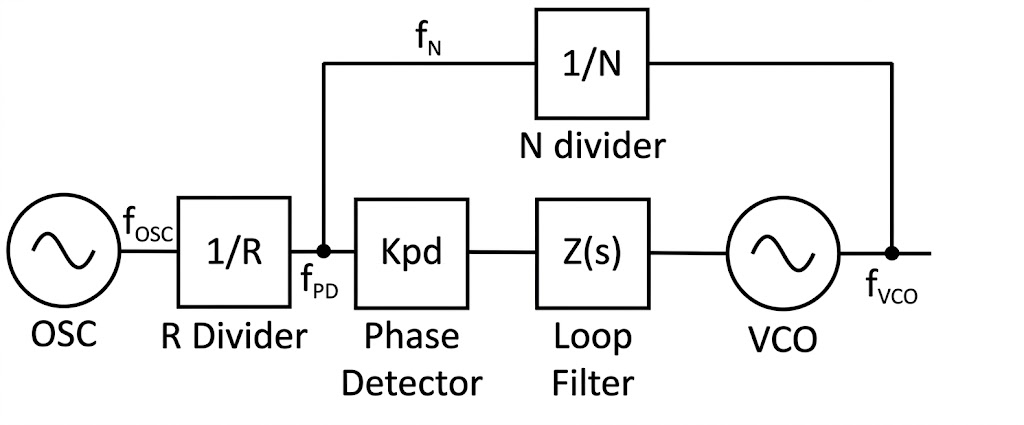
\includegraphics[width=0.75\linewidth]{imagenes/PLL diagrama bloque.png}
    \caption{Diagrama básico del PLL. (Fuente: \cite{Dean Banerjee}).}
    \label{fig:fig4.1}
\end{figure}

El filtro de bucle tiene la función de controlar la frecuencia de salida del oscilador controlado por voltaje (VCO, por sus siglas en inglés). Este dispositivo actúa como un convertidor de voltaje a frecuencia, el cual está caracterizado por una constante de proporcionalidad $K_{VCO}$.

Posteriormente, la señal de salida del VCO atraviesa el divisor $N$, el cual reduce su frecuencia hasta adaptarla a la entrada del detector de fase ($f_N$).

El detector se encarga de comparar las fases de ambas señales de entrada. Al alcanzar el estado estacionario, estas entradas igualan tanto su frecuencia como su fase, dando como resultado que la frecuencia del VCO sea la siguiente:
\begin{equation}
    f_{VCO} = f_{OSC} \cdot \frac{N}{R}
\end{equation}

El valor del divisor $N$ se puede modificar para obtener un rango de frecuencias VCO con la misma precisión que el cristal. Al especificar un rango, normalmente se indica un espaciado de canal $f_{CH}$ para la separación entre las frecuencias. Generalmente, se busca maximizar la frecuencia del detector de fase, lo que implica que se elegiría igual al espaciado de canal en este caso, a menos que existan otras restricciones en el dispositivo que obliguen a elegir un valor inferior.

Si la frecuencia de salida del PLL es fija, la elección del valor del divisor $N$ puede no ser intuitivamente obvia, ya que existen muchas opciones. En este caso, lo ideal es elegir el divisor $N$ más pequeño posible para maximizar la frecuencia del detector de fase y obtener así el mejor rendimiento en cuanto a ruido. En el caso de que exista libertad para elegir la frecuencia de referencia de entrada, es mejor elegirla de manera que tenga muchos factores comunes con la frecuencia de salida para que el valor de $N$ sea lo más pequeño posible.

El término PLL se refiere técnicamente al sistema completo que se muestra en la Figura~\ref{fig:fig4.1}; sin embargo, las dificultades para integrar el VCO y la señal de entrada han llevado a la industria a redefinir el término. A menudo, cuando se compra un chip ``PLL'' a los fabricantes de semiconductores, este solo incluye los divisores y la bomba de carga. Cuando surgió la capacidad de integrar VCOs, los proveedores de semiconductores no quisieron denominarlo PLL porque querían dejar claro que el VCO también estaba incluido; por lo tanto, a menudo se le llama sintetizador de frecuencia \cite{Dean Banerjee}.

\section{Características del bucle}
La función de transferencia de lazo cerrado, desde la entrada del detector de fase hasta la salida del VCO, está determinada por el divisor $N$, la ganancia del VCO, la ganancia de la bomba de carga y el filtro de lazo. Se trata de una función de paso bajo cuya frecuencia de corte se denomina ancho de banda del lazo ($BW$).

La elección de este ancho de banda es el parámetro de diseño más crítico, ya que tiene un impacto significativo en el ruido de fase, las señales espurias y la velocidad de conmutación del PLL.

Para todo el ruido y las espurias que no provienen del VCO, esta función de transferencia multiplica el ruido de fase dentro del ancho de banda del lazo; posteriormente, la atenuación del filtro comienza a actuar por encima de esta frecuencia. Por otro lado, en el caso del ruido generado por el propio VCO, este se suprime por debajo de la frecuencia del ancho de banda del lazo y se mantiene inalterado por encima de ella \cite{Dean Banerjee}.

\begin{figure}[H]
    \centering
    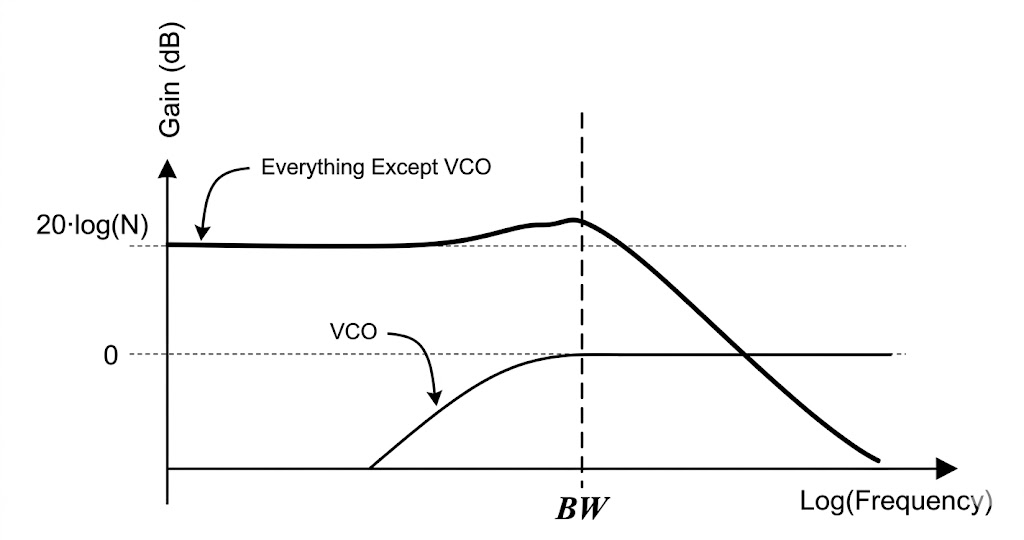
\includegraphics[width=1\linewidth]{imagenes/respuesta bucle y VCO.png}
    \caption{Bucle del PLL. (Fuente: \cite{Dean Banerjee}).}
    \label{fig:fig4.2}
\end{figure}

\subsection{Ruido de fase del PLL}
Además de la señal deseada, un PLL también genera ruido no deseado. Este ruido se puede considerar como ruido de fase en la señal de salida y, por lo tanto, se denomina ruido de fase. En el dominio de la frecuencia, se suele expresar como la densidad de potencia del ruido en relación con la potencia de la portadora y se mide en dBc/Hz, como se muestra a continuación en la Figura~\ref{fig:fig4.2_ruido}.

\begin{figure}[H]
    \centering
    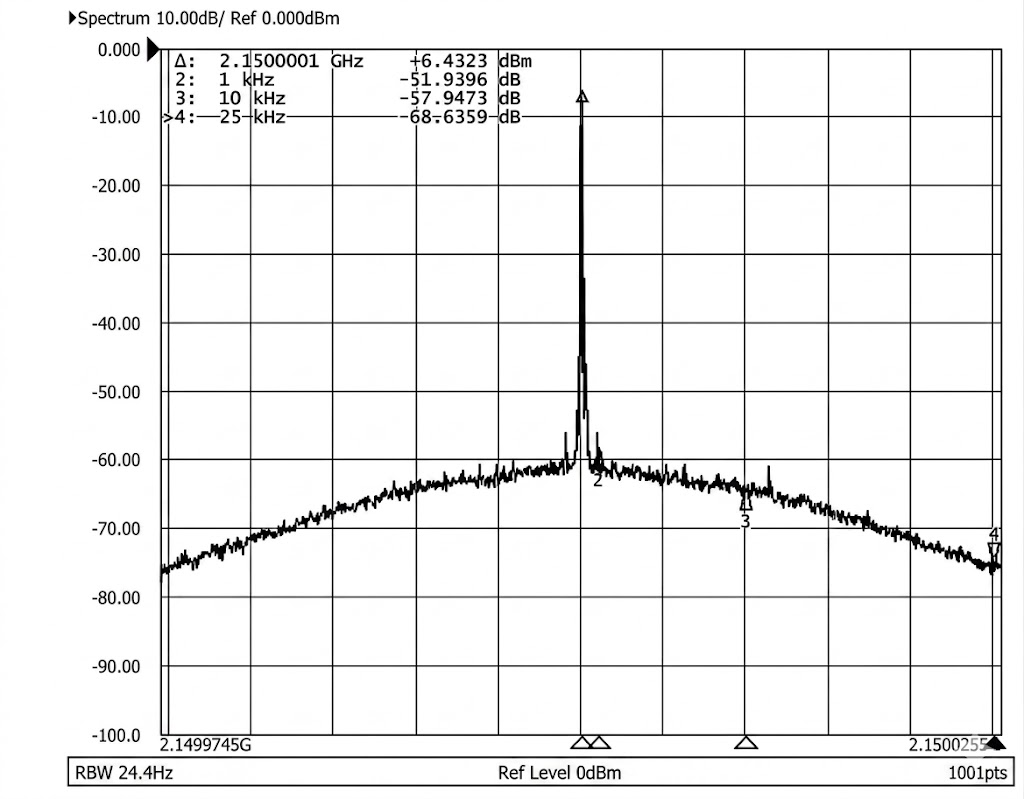
\includegraphics[width=1\linewidth]{imagenes/imagen teórica ruido de fase.png}
    \caption{Ruido de fase del PLL. (Fuente: \cite{Dean Banerjee}).}
    \label{fig:fig4.2_ruido}
\end{figure}

Para poder calcular el ruido de fase en el analizador de espectro se debe tener en cuenta el ancho de la ventana, ya que es una medición que se realiza por unidad de frecuencia \cite{Dean Banerjee}:
\begin{equation}
\mathcal{L}(f_m) = P_N(f_m) - P_C - 10\log_{10}(RBW)
\end{equation}

\subsection{Espurios del PLL}
Las espurias pueden considerarse como ruido concentrado en un desplazamiento específico respecto a la portadora, como se muestra en la Figura~\ref{fig:fig4.3}. Suelen medirse en dBc con un analizador de espectro. Existen muchos tipos de espurias y pueden tener múltiples causas, pero la mayoría se producen en desplazamientos muy predecibles. Las espurias tienden a aparecer en múltiplos de la frecuencia del detector de fase, la frecuencia de referencia de entrada, el espaciado entre canales y fracciones de este.

\begin{figure}[H]
    \centering
    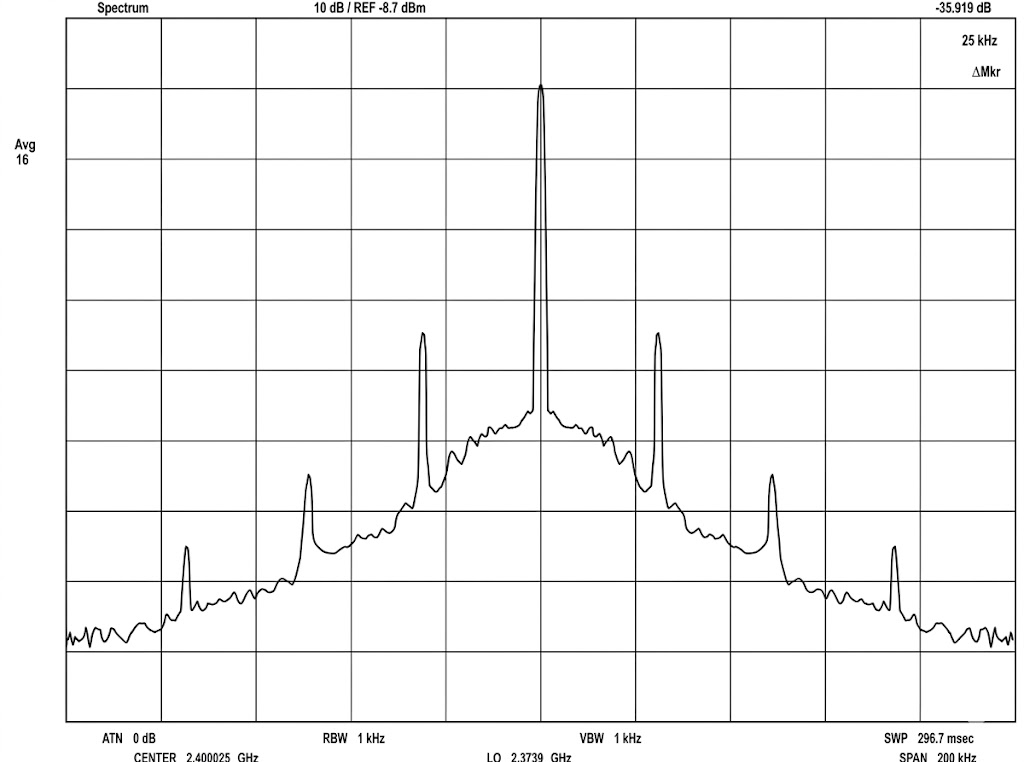
\includegraphics[width=1\linewidth]{imagenes/Spurios teorico.png}
    \caption{Espurios del PLL. (Fuente: \cite{Dean Banerjee}).}
    \label{fig:fig4.3}
\end{figure}

El ruido de fase, las espurias y el tiempo de enganche son características clave de rendimiento y se ven afectadas drásticamente por las características del bucle, especialmente por su ancho de banda. Un ancho de banda menor tiende a reducir las espurias y el ruido de fase lejano, pero aumenta el tiempo de enganche. Lo contrario ocurre con un ancho de banda amplio, aunque este puede mejorar el ruido de fase cercano según la calidad del ruido de la referencia de entrada. Las distintas aplicaciones pueden tener requisitos diferentes, por lo que no existe un diseño de PLL óptimo para todas ellas \cite{Dean Banerjee}.

\section{Bloques del PLL}
Como se mostró en la Figura~\ref{fig:fig4.1}, el PLL consta de distintos bloques para lograr su funcionamiento. Es importante saber para qué se utiliza cada uno de ellos, los cuales se detallan a continuación:

\subsection{Referencia de oscilación}
El PLL parte de la premisa de que existe una señal de entrada. Esta debe tener una frecuencia muy precisa, ya que cualquier error se transmite directamente al VCO. Dicha señal puede ser un reloj recuperado, una frecuencia generada por otro chip o una señal generada por un cristal u oscilador de cristal. No es infrecuente que los osciladores de cristal alcancen precisiones de frecuencia de diez partes por millón.

La principal causa de error de frecuencia en estos osciladores es la deriva térmica. El oscilador de cristal con compensación de temperatura (TCXO) incorpora un sensor de temperatura y un sistema de compensación para corregir la frecuencia del cristal en función de la temperatura. Esto mejora la precisión de la frecuencia en aproximadamente un factor de diez. El oscilador de cristal controlado por horno (OCXO) mejora el rendimiento aproximadamente en un factor de diez al hacer que un horno caliente el cristal a una temperatura constante \cite{Dean Banerjee}.

\begin{table}[h!]
\centering
\renewcommand{\arraystretch}{1.5}
\begin{tabular}{|c|>{\raggedright\arraybackslash}p{4.2cm}|c|>{\raggedright\arraybackslash}p{6cm}|}
\hline
\textbf{Acrónimo} & \textbf{Tipo de Oscilador} & \textbf{Precisión} & \textbf{Comentarios} \\
\hline
XO & Oscilador de cristal & 10 ppm & Esto es un cristal más el inversor. \\
\hline
TCXO & Oscilador de cristal compensado por temperatura & 1 ppm & Utiliza circuitos para compensar la frecuencia según la temperatura, pero a veces estos circuitos pueden añadir ruido. \\
\hline
VCXO & Oscilador de cristal compensado por voltaje & 10 ppm & Como un oscilador de cristal, pero se puede utilizar un voltaje para ajustar la frecuencia. \\
\hline
OCXO & Oscilador de cristal controlado por horno & 0.1 ppm & Utiliza un horno para mantener una temperatura constante. \\
\hline
\end{tabular}
\caption{Tipos de Osciladores}
\label{tab:tipos_osciladores}
\end{table}

\subsection{Divisor R}
Aunque la ruta de entrada y el divisor $R$ no parezcan los bloques más complejos del PLL, merecen ser analizados, ya que la salida de este bloque se multiplica mediante el divisor $N$ para llegar a la salida del VCO. Si este bloque es ruidoso o si la señal de entrada no tiene una velocidad de respuesta suficiente, pueden producirse degradaciones en los espurios y el ruido de fase. Cuando la frecuencia de entrada ($f_{OSC}$) es una onda sinusoidal de baja frecuencia, esto tiende a generar velocidades de respuesta más lentas en la señal, lo que puede afectar el rendimiento del PLL. 

La ruta de entrada también puede ser más sofisticada e incluir duplicadores y multiplicadores. Algunos dispositivos ofrecen multiplicadores de entrada programables para mejorar el ruido de fase o las espurias del PLL. Sin embargo, hay que tener en cuenta que estos bloques pueden añadir ruido. Los duplicadores son más fáciles de implementar, por lo que a menudo no añaden ruido perceptible. Los multiplicadores mayores que dos pueden añadir una cantidad significativa de ruido, y la cantidad de ruido añadido depende del dispositivo \cite{Dean Banerjee}.

\subsection{El detector de fase y la bomba de carga}
El detector de fase es un dispositivo que convierte las diferencias de fase entre el contador $N$ y el contador $R$ en una tensión de salida. Esta tensión puede aplicarse directamente al filtro de bucle o convertirse en corriente mediante la bomba de carga \cite{Dean Banerjee}.

\subsubsection{El detector de fase de voltaje}
El detector de fase de voltaje era el método comúnmente utilizado antes de la introducción de la bomba de carga y genera un voltaje proporcional al error de fase entre las salidas de los divisores $N$ y $R$. Puede implementarse con un mezclador, una puerta XOR o un flip-flop JK. Quizás la razón por la que el detector de fase de voltaje perdió popularidad en comparación con la bomba de carga fue su incapacidad para lograr y mantener la sincronización si la frecuencia/fase del VCO se desviaba demasiado del valor objetivo.

\subsubsection{Detector de fase/frecuencia (PFD) y la bomba de carga}
La combinación de detector de fase/frecuencia (PFD) y bomba de carga ha reemplazado al detector de voltaje en muchos diseños, ya que no presenta problemas para obtener y mantener la sincronización y no requiere componentes activos.

El detector de fase (PFD) compara las salidas de los contadores $N$ y $R$ para generar una tensión de corrección, que la bomba de carga convierte en corriente. En la Figura~\ref{fig:fig4.5} se muestra la estructura simplificada del PFD y la bomba de carga.

\begin{figure}[H]
    \centering
    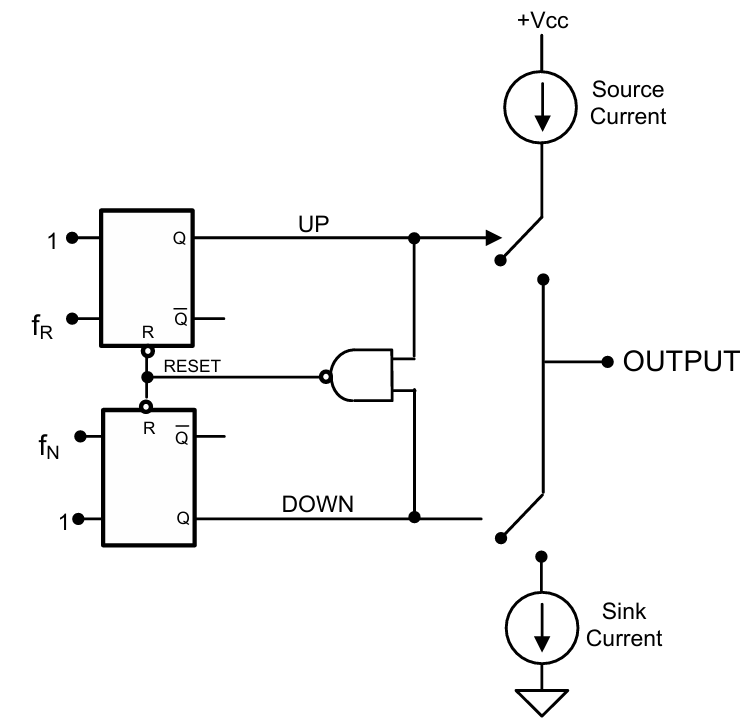
\includegraphics[width=0.65\linewidth]{imagenes/detector de fase y bomba de carga.png}
    \caption{Detector de fase/frecuencia y bomba de carga. (Fuente: \cite{Dean Banerjee}).}
    \label{fig:fig4.5}
\end{figure}

En la Figura~\ref{fig:fig4.5} se muestra una implementación del PFD y la bomba de carga, donde $f_N$ representa la señal del divisor $N$ y $f_R$ la del divisor $R$. El circuito presenta tres estados posibles: corriente de fuente habilitada, corriente de sumidero habilitada o ambas corrientes deshabilitadas. Sin embargo, no se permite el estado de ambas corrientes habilitadas, ya que si las señales UP y DOWN estuvieran en nivel alto, se reiniciarían los flip-flops, provocando que ambos interruptores se abrieran.

Se dice que el circuito de la Figura~\ref{fig:fig4.5} tiene polaridad positiva en el detector de fase porque un error de fase positivo genera una corriente de corrección positiva. En muchos PLL, es posible invertir la polaridad del detector de fase, de modo que se invierta el comportamiento entre las corrientes de sumidero y fuente. Cuando se realiza esta inversión, se dice que el detector de fase tiene polaridad negativa. Esta característica suele ser útil al usar filtros activos.

Aumentar el ancho de banda del bucle más allá de una décima parte de la frecuencia del detector de fase podría no producir la mejora esperada en el tiempo de sincronización. Además, las espurias podrían tener un efecto de cúspide debido a este muestreo. Si el ancho de banda del bucle es inferior a aproximadamente 1/100 de la frecuencia del detector de fase, el tiempo de sincronización podría degradarse debido al deslizamiento de ciclo.

\subsection{Filtro de lazo}
\label{subsec:filtrolazomarco}
El filtro de bucle es un filtro paso bajo que convierte la corriente de salida de la bomba de carga en una tensión de sintonización para el VCO. Sin embargo, no sirve cualquier filtro paso bajo. La función de transferencia del filtro de bucle forma parte del PLL de lazo cerrado, que también incluye el valor del divisor $N$, la ganancia de la bomba de carga y la ganancia del VCO. Esta función de transferencia de bucle cerrado tiene un profundo impacto en la velocidad de conmutación del PLL, las espurias, el ruido de fase y la estabilidad.

En general, lo ideal es implementar el filtro de bucle con resistencias y condensadores por razones de costo y ruido. Sin embargo, en algunas situaciones puede ser necesario utilizar un dispositivo activo como un amplificador operacional. La razón más común para esto es cuando la bomba de carga no puede generar un voltaje suficientemente alto \cite{Dean Banerjee}.

\begin{figure}[H]
    \centering
    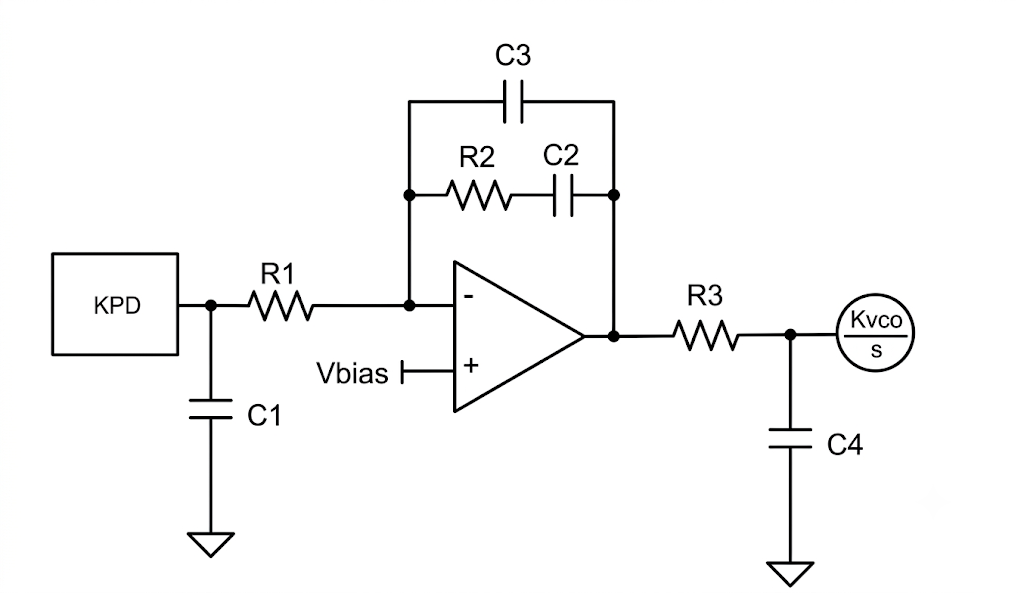
\includegraphics[width=0.75\linewidth]{imagenes/filtro de lazo.png}
    \caption{Filtro de bucle activo. (Fuente: \cite{Dean Banerjee}).}
    \label{fig:fig4.6}
\end{figure}

\subsubsection{Análisis del filtro de lazo}

Suponiendo un amplificador operacional ideal, la entrada inversora se encuentra en tierra virtual y no circula corriente hacia sus terminales de entrada. La función de transferencia del filtro activo es:

\begin{equation}
H(s) = \frac{V_o(s)}{V_i(s)} = -\frac{Z_f(s)}{R_1},
\end{equation}

donde $Z_f(s)$ es la impedancia equivalente de la red de realimentación.

La red de realimentación está formada por dos ramas en paralelo:

\begin{equation}
Z_{C_3} = \frac{1}{sC_3},
\end{equation}

y

\begin{equation}
Z_{R_2C_2} = R_2 + \frac{1}{sC_2}.
\end{equation}

Por lo tanto,

\begin{equation}
Z_f = \left(\frac{1}{Z_{C_3}} + \frac{1}{Z_{R_2C_2}}\right)^{-1}.
\end{equation}

Sustituyendo,

\begin{equation}
Z_f = \left(sC_3 + \frac{1}{R_2 + \dfrac{1}{sC_2}}\right)^{-1}.
\end{equation}

La segunda admitancia puede escribirse como:

\begin{equation}
\frac{1}{R_2 + \dfrac{1}{sC_2}} = \frac{sC_2}{1 + sR_2C_2}.
\end{equation}

Entonces,

\begin{equation}
Z_f = \left(sC_3 + \frac{sC_2}{1 + sR_2C_2}\right)^{-1}.
\end{equation}

Llevando ambas admitancias al mismo denominador,

\begin{equation}
Z_f = \frac{1 + sR_2C_2}{s(C_2 + C_3) + s^2R_2C_2C_3}.
\end{equation}

Finalmente, la función de transferencia queda:

\begin{equation}
H(s) = -\frac{1 + sR_2C_2}{R_1\left[s(C_2 + C_3) + s^2R_2C_2C_3\right]}.
\end{equation}

Factorizando el denominador,

\begin{equation}
H(s) = -\frac{1}{R_1(C_2 + C_3)} \frac{1 + sR_2C_2}{s\left(1 + s\dfrac{R_2C_2C_3}{C_2 + C_3}\right)}.
\end{equation}

\subsubsection{Polos adicionales del modelo del PLL}

El modelo completo utilizado por ADIsimPLL incorpora además los siguientes polos:

\begin{itemize}
\item Polo debido al filtro de salida:
\begin{equation}
\omega_{p3} = \frac{1}{R_3(C_4 + C_{VCO})},
\end{equation}
donde $C_{VCO}$ representa la capacitancia de entrada del VCO.

\item Polo debido al filtro de entrada de la bomba de carga:
\begin{equation}
\omega_{p4} = \frac{1}{R_1C_1}.
\end{equation}
\end{itemize}

\subsubsection{Polos y ceros}

La función de transferencia presenta un cero y dos polos:

\begin{itemize}
\item Cero:
\begin{equation}
\omega_z = \frac{1}{R_2C_2}.
\end{equation}

\item Polo en el origen:
\begin{equation}
\omega_{p1} = 0.
\end{equation}

\item Segundo polo:
\begin{equation}
\omega_{p2} = \frac{C_2 + C_3}{R_2C_2C_3}.
\end{equation}
\end{itemize}

\subsection{Voltage Controlled Oscillators (VCO)}

El oscilador controlado por voltaje (VCO) genera una frecuencia basada en el voltaje de entrada. Puede considerarse un convertidor de voltaje a frecuencia \cite{Dean Banerjee}.

\subsubsection{Rango de frecuencia y sintonización}
Un rango de frecuencias más amplio siempre es deseable, pero esto conlleva un aumento del ruido de fase. La frecuencia mínima se define como $f_{\text{VCOmin}}$ y se obtiene con una tensión de entrada de $V_{\text{TuneMin}}$. La frecuencia máxima se define como $f_{\text{VCOmax}}$ y se obtiene con una tensión de entrada de $V_{\text{TuneMax}}$.

\subsubsection{Ganancia del VCO}
La ganancia del VCO, $K_{\text{VCO}}$, se expresa en MHz/V e indica cuánto cambia la frecuencia de salida ante un cambio en la tensión de entrada. Es deseable que esta ganancia sea constante en todo el rango de sintonización del VCO.
\begin{equation}
K_{\text{VCO}} = \frac{df_{\text{VCO}}}{dV_{\text{Tune}}} \approx \frac{f_{\text{VCOmax}} - f_{\text{VCOmin}}}{V_{\text{TuneMax}} - V_{\text{TuneMin}}}
\end{equation}

La ganancia del VCO se puede calcular a partir de la pendiente de la curva de sintonización. Si es constante, se puede calcular para todo el rango. Si no, se puede calcular evaluando la pendiente de la curva de sintonización en un rango pequeño alrededor de cada voltaje $V_{\text{Tune}}$ o dividiendo el rango de sintonización del VCO en varias regiones \cite{Dean Banerjee}.

\subsection{Función de transferencia}
Teniendo en cuenta el filtro de lazo activo analizado en la Figura~\ref{fig:fig4.6}, se puede hacer un análisis de las funciones de transferencia a lazo abierto y cerrado.

\subsubsection{Función de transferencia a lazo abierto}

La función de transferencia de lazo abierto de todo el lazo del PLL se define como el producto de las funciones de transferencia correspondientes a cada uno de los bloques que conforman la trayectoria directa y de realimentación del lazo. Incorpora el detector de fase (PFD), el filtro de lazo, el VCO y el divisor $N$:

\begin{equation}
G(s) = \frac{K_{\mathrm{PFD}} K_{\mathrm{VCO,rad}}}{N \cdot s} F(s).
\end{equation}

El factor $1/s$ evidencia que el VCO actúa como un integrador ideal, convirtiendo la frecuencia de salida en fase. Sustituyendo la expresión completa del filtro de lazo y la constante de ganancia $K_F$:

\begin{equation}
G(s) = \frac{K_{\mathrm{PFD}} K_{\mathrm{VCO,rad}}}{N} K_F \frac{1 + s/\omega_z}{s^2 \left(1 + s/\omega_{p2}\right) \left(1 + s/\omega_{p3}\right) \left(1 + s/\omega_{p4}\right)}.
\end{equation}

La presencia del término $s^2$ en el denominador indica la existencia de dos integradores en el lazo (uno asociado al filtro y otro al VCO). Esto le confiere al PLL un comportamiento de tipo II, el cual es ideal para seguir variaciones dinámicas como rampas de frecuencia (FMCW) \cite{Dean Banerjee}.

\subsubsection{Función de transferencia a lazo cerrado}

La función de transferencia a lazo cerrado $CL(s)$ modela la respuesta del sistema completo. Considerando que la trayectoria de realimentación está dada por el divisor $H = 1/N$ y la ganancia de la trayectoria directa es $G_{fwd}(s) = N \cdot G(s)$, la transferencia resulta en \cite{Dean Banerjee}:

\begin{equation}
CL(s) = \frac{N \cdot G(s)}{1 + G(s)}.
\end{equation}

Para simplificar su evaluación, la función de lazo abierto $G(s)$ puede expresarse como el cociente entre un numerador $\text{Num}(s)$ y un denominador $\text{Den}(s)$. De esta manera, la función de lazo cerrado se reescribe como:

\begin{equation}
CL(s) = N \frac{\text{Num}(s)}{\text{Den}(s) + \text{Num}(s)}.
\end{equation}

Las raíces de este polinomio corresponden a los polos a lazo cerrado del sistema, los cuales determinan en última instancia la estabilidad absoluta, el tiempo de enganche (\textit{lock time}) y la dinámica transitoria para la generación de la modulación FMCW.

\subsubsection{Ancho de banda del lazo y margen de fase}

El ancho de banda del lazo se define como la frecuencia para la cual la magnitud de la función de transferencia de lazo abierto es igual a la unidad. Matemáticamente:

\begin{equation}
\left|G(j\omega_c)\right| = 1,
\label{eq:bw1}
\end{equation}

donde $\omega_c$ es la frecuencia de cruce de ganancia (\textit{loop bandwidth}) expresada en rad/s.

La relación entre la frecuencia angular y la frecuencia en Hertz es:

\begin{equation}
\omega_c = 2\pi BW,
\label{eq:bw2}
\end{equation}

donde $BW$ representa el ancho de banda del lazo en Hz.

El margen de fase se define como la diferencia entre $180^\circ$ y la fase de la función de transferencia de lazo abierto evaluada en la frecuencia de cruce de ganancia:

\begin{equation}
PM = 180^\circ + \angle G(j\omega_c).
\label{eq:pm}
\end{equation}